% Created by tikzDevice version 0.12.6 on 2026-05-16 21:30:22
% !TEX encoding = UTF-8 Unicode
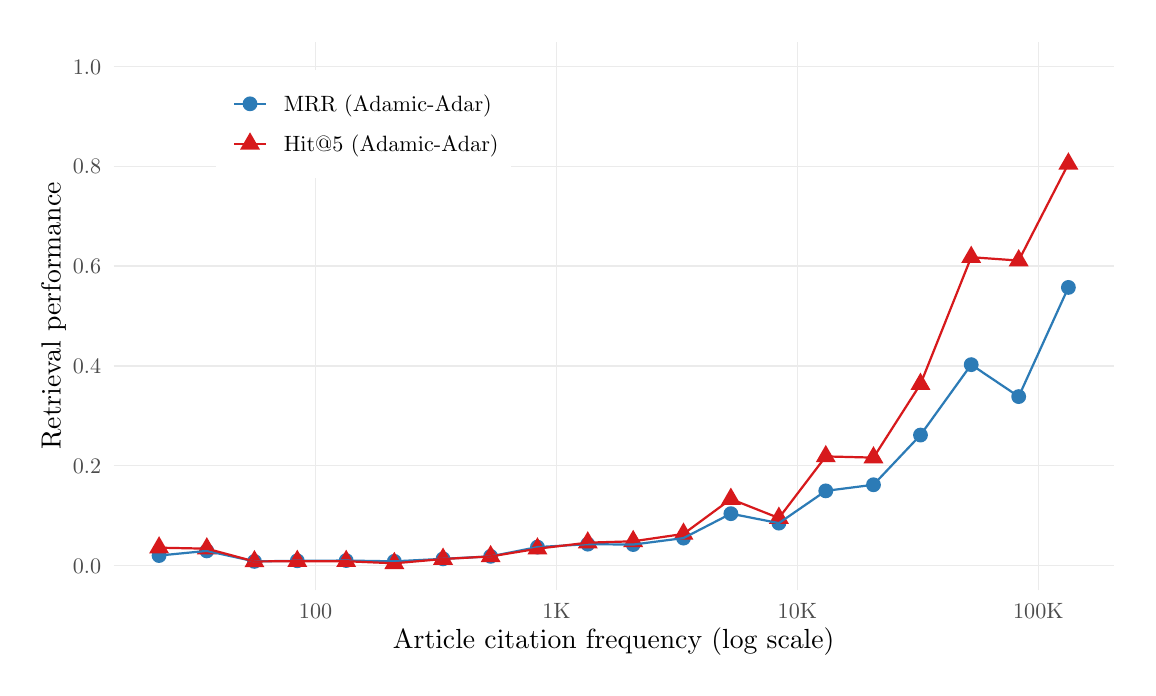
\begin{tikzpicture}[x=1pt,y=1pt]
\definecolor{fillColor}{RGB}{255,255,255}
\path[use as bounding box,fill=fillColor,fill opacity=0.00] (0,0) rectangle (397.48,231.26);
\begin{scope}
\path[clip] (  0.00,  0.00) rectangle (397.48,231.26);
\definecolor{fillColor}{RGB}{255,255,255}

\path[fill=fillColor] (  0.00,  0.00) rectangle (397.48,231.26);
\end{scope}
\begin{scope}
\path[clip] ( 31.05, 27.90) rectangle (392.48,226.26);
\definecolor{drawColor}{gray}{0.92}

\path[draw=drawColor,line width= 0.5pt,line join=round] ( 31.05, 36.91) --
	(392.48, 36.91);

\path[draw=drawColor,line width= 0.5pt,line join=round] ( 31.05, 72.98) --
	(392.48, 72.98);

\path[draw=drawColor,line width= 0.5pt,line join=round] ( 31.05,109.05) --
	(392.48,109.05);

\path[draw=drawColor,line width= 0.5pt,line join=round] ( 31.05,145.11) --
	(392.48,145.11);

\path[draw=drawColor,line width= 0.5pt,line join=round] ( 31.05,181.18) --
	(392.48,181.18);

\path[draw=drawColor,line width= 0.5pt,line join=round] ( 31.05,217.25) --
	(392.48,217.25);

\path[draw=drawColor,line width= 0.5pt,line join=round] (104.03, 27.90) --
	(104.03,226.26);

\path[draw=drawColor,line width= 0.5pt,line join=round] (191.09, 27.90) --
	(191.09,226.26);

\path[draw=drawColor,line width= 0.5pt,line join=round] (278.14, 27.90) --
	(278.14,226.26);

\path[draw=drawColor,line width= 0.5pt,line join=round] (365.20, 27.90) --
	(365.20,226.26);
\definecolor{fillColor}{RGB}{44,123,182}

\path[fill=fillColor] ( 47.48, 40.51) circle (  2.68);

\path[fill=fillColor] ( 64.73, 42.19) circle (  2.68);

\path[fill=fillColor] ( 81.94, 38.40) circle (  2.68);

\path[fill=fillColor] ( 97.42, 38.62) circle (  2.68);

\path[fill=fillColor] (115.09, 38.70) circle (  2.68);

\path[fill=fillColor] (132.49, 38.42) circle (  2.68);

\path[fill=fillColor] (150.09, 39.32) circle (  2.68);

\path[fill=fillColor] (167.29, 40.22) circle (  2.68);

\path[fill=fillColor] (184.20, 43.56) circle (  2.68);

\path[fill=fillColor] (202.39, 44.62) circle (  2.68);

\path[fill=fillColor] (218.80, 44.48) circle (  2.68);

\path[fill=fillColor] (236.98, 46.82) circle (  2.68);

\path[fill=fillColor] (254.10, 55.64) circle (  2.68);

\path[fill=fillColor] (271.45, 52.22) circle (  2.68);

\path[fill=fillColor] (288.39, 63.88) circle (  2.68);

\path[fill=fillColor] (305.63, 66.09) circle (  2.68);

\path[fill=fillColor] (322.61, 84.05) circle (  2.68);

\path[fill=fillColor] (340.94,109.49) circle (  2.68);

\path[fill=fillColor] (358.10, 97.95) circle (  2.68);

\path[fill=fillColor] (376.06,137.40) circle (  2.68);
\definecolor{fillColor}{RGB}{215,25,28}

\path[fill=fillColor] ( 47.48, 47.52) --
	( 51.09, 41.27) --
	( 43.87, 41.27) --
	cycle;

\path[fill=fillColor] ( 64.73, 47.17) --
	( 68.34, 40.92) --
	( 61.12, 40.92) --
	cycle;

\path[fill=fillColor] ( 81.94, 42.54) --
	( 85.55, 36.29) --
	( 78.33, 36.29) --
	cycle;

\path[fill=fillColor] ( 97.42, 42.65) --
	(101.03, 36.40) --
	( 93.81, 36.40) --
	cycle;

\path[fill=fillColor] (115.09, 42.63) --
	(118.70, 36.38) --
	(111.49, 36.38) --
	cycle;

\path[fill=fillColor] (132.49, 41.88) --
	(136.10, 35.63) --
	(128.88, 35.63) --
	cycle;

\path[fill=fillColor] (150.09, 43.42) --
	(153.70, 37.17) --
	(146.48, 37.17) --
	cycle;

\path[fill=fillColor] (167.29, 44.36) --
	(170.90, 38.11) --
	(163.68, 38.11) --
	cycle;

\path[fill=fillColor] (184.20, 47.15) --
	(187.81, 40.90) --
	(180.59, 40.90) --
	cycle;

\path[fill=fillColor] (202.39, 49.33) --
	(206.00, 43.08) --
	(198.78, 43.08) --
	cycle;

\path[fill=fillColor] (218.80, 49.83) --
	(222.41, 43.57) --
	(215.19, 43.57) --
	cycle;

\path[fill=fillColor] (236.98, 52.49) --
	(240.59, 46.24) --
	(233.37, 46.24) --
	cycle;

\path[fill=fillColor] (254.10, 65.09) --
	(257.71, 58.84) --
	(250.49, 58.84) --
	cycle;

\path[fill=fillColor] (271.45, 58.24) --
	(275.05, 51.99) --
	(267.84, 51.99) --
	cycle;

\path[fill=fillColor] (288.39, 80.50) --
	(292.00, 74.25) --
	(284.78, 74.25) --
	cycle;

\path[fill=fillColor] (305.63, 80.07) --
	(309.24, 73.82) --
	(302.02, 73.82) --
	cycle;

\path[fill=fillColor] (322.61,106.62) --
	(326.22,100.37) --
	(319.00,100.37) --
	cycle;

\path[fill=fillColor] (340.94,152.49) --
	(344.55,146.24) --
	(337.33,146.24) --
	cycle;

\path[fill=fillColor] (358.10,151.27) --
	(361.71,145.02) --
	(354.49,145.02) --
	cycle;

\path[fill=fillColor] (376.06,186.25) --
	(379.66,180.00) --
	(372.45,180.00) --
	cycle;
\definecolor{drawColor}{RGB}{44,123,182}

\path[draw=drawColor,line width= 0.8pt,line join=round] ( 47.48, 40.51) --
	( 64.73, 42.19) --
	( 81.94, 38.40) --
	( 97.42, 38.62) --
	(115.09, 38.70) --
	(132.49, 38.42) --
	(150.09, 39.32) --
	(167.29, 40.22) --
	(184.20, 43.56) --
	(202.39, 44.62) --
	(218.80, 44.48) --
	(236.98, 46.82) --
	(254.10, 55.64) --
	(271.45, 52.22) --
	(288.39, 63.88) --
	(305.63, 66.09) --
	(322.61, 84.05) --
	(340.94,109.49) --
	(358.10, 97.95) --
	(376.06,137.40);
\definecolor{drawColor}{RGB}{215,25,28}

\path[draw=drawColor,line width= 0.8pt,line join=round] ( 47.48, 43.35) --
	( 64.73, 43.00) --
	( 81.94, 38.38) --
	( 97.42, 38.48) --
	(115.09, 38.46) --
	(132.49, 37.71) --
	(150.09, 39.26) --
	(167.29, 40.19) --
	(184.20, 42.98) --
	(202.39, 45.17) --
	(218.80, 45.66) --
	(236.98, 48.32) --
	(254.10, 60.92) --
	(271.45, 54.07) --
	(288.39, 76.33) --
	(305.63, 75.90) --
	(322.61,102.45) --
	(340.94,148.32) --
	(358.10,147.10) --
	(376.06,182.08);
\end{scope}
\begin{scope}
\path[clip] (  0.00,  0.00) rectangle (397.48,231.26);
\definecolor{drawColor}{gray}{0.30}

\node[text=drawColor,anchor=base east,inner sep=0pt, outer sep=0pt, scale=  0.80] at ( 26.55, 34.16) {0.0};

\node[text=drawColor,anchor=base east,inner sep=0pt, outer sep=0pt, scale=  0.80] at ( 26.55, 70.22) {0.2};

\node[text=drawColor,anchor=base east,inner sep=0pt, outer sep=0pt, scale=  0.80] at ( 26.55,106.29) {0.4};

\node[text=drawColor,anchor=base east,inner sep=0pt, outer sep=0pt, scale=  0.80] at ( 26.55,142.36) {0.6};

\node[text=drawColor,anchor=base east,inner sep=0pt, outer sep=0pt, scale=  0.80] at ( 26.55,178.43) {0.8};

\node[text=drawColor,anchor=base east,inner sep=0pt, outer sep=0pt, scale=  0.80] at ( 26.55,214.49) {1.0};
\end{scope}
\begin{scope}
\path[clip] (  0.00,  0.00) rectangle (397.48,231.26);
\definecolor{drawColor}{gray}{0.30}

\node[text=drawColor,anchor=base,inner sep=0pt, outer sep=0pt, scale=  0.80] at (104.03, 17.89) {100};

\node[text=drawColor,anchor=base,inner sep=0pt, outer sep=0pt, scale=  0.80] at (191.09, 17.89) {1K};

\node[text=drawColor,anchor=base,inner sep=0pt, outer sep=0pt, scale=  0.80] at (278.14, 17.89) {10K};

\node[text=drawColor,anchor=base,inner sep=0pt, outer sep=0pt, scale=  0.80] at (365.20, 17.89) {100K};
\end{scope}
\begin{scope}
\path[clip] (  0.00,  0.00) rectangle (397.48,231.26);
\definecolor{drawColor}{RGB}{0,0,0}

\node[text=drawColor,anchor=base,inner sep=0pt, outer sep=0pt, scale=  1.00] at (211.77,  6.94) {Article citation frequency (log scale)};
\end{scope}
\begin{scope}
\path[clip] (  0.00,  0.00) rectangle (397.48,231.26);
\definecolor{drawColor}{RGB}{0,0,0}

\node[text=drawColor,rotate= 90.00,anchor=base,inner sep=0pt, outer sep=0pt, scale=  1.00] at ( 11.89,127.08) {Retrieval performance};
\end{scope}
\begin{scope}
\path[clip] (  0.00,  0.00) rectangle (397.48,231.26);
\definecolor{fillColor}{RGB}{255,255,255}

\path[fill=fillColor] ( 68.13,177.05) rectangle (174.69,215.96);
\end{scope}
\begin{scope}
\path[clip] (  0.00,  0.00) rectangle (397.48,231.26);
\definecolor{fillColor}{RGB}{44,123,182}

\path[fill=fillColor] ( 80.35,203.74) circle (  2.68);
\definecolor{drawColor}{RGB}{44,123,182}

\path[draw=drawColor,line width= 0.8pt,line join=round] ( 74.57,203.74) -- ( 86.13,203.74);
\end{scope}
\begin{scope}
\path[clip] (  0.00,  0.00) rectangle (397.48,231.26);
\definecolor{fillColor}{RGB}{215,25,28}

\path[fill=fillColor] ( 80.35,193.45) --
	( 83.96,187.20) --
	( 76.74,187.20) --
	cycle;
\definecolor{drawColor}{RGB}{215,25,28}

\path[draw=drawColor,line width= 0.8pt,line join=round] ( 74.57,189.28) -- ( 86.13,189.28);
\end{scope}
\begin{scope}
\path[clip] (  0.00,  0.00) rectangle (397.48,231.26);
\definecolor{drawColor}{RGB}{0,0,0}

\node[text=drawColor,anchor=base west,inner sep=0pt, outer sep=0pt, scale=  0.80] at ( 92.58,200.98) {MRR (Adamic-Adar)};
\end{scope}
\begin{scope}
\path[clip] (  0.00,  0.00) rectangle (397.48,231.26);
\definecolor{drawColor}{RGB}{0,0,0}

\node[text=drawColor,anchor=base west,inner sep=0pt, outer sep=0pt, scale=  0.80] at ( 92.58,186.53) {Hit@5 (Adamic-Adar)};
\end{scope}
\end{tikzpicture}
